\documentclass{article}

\usepackage{../.template/summary}

\subject{Privacy by Design}
\semester{Winter 2024}
\author{Leopold Lemmermann}

\usepackage{pdfpages}

\begin{document}\createtitle

\includepdf[pages={23-24, 27-39, 41-57, 59-124}, nup=4x9]{slides.pdf}
\part{Privacy Enhancing Technology}
\section{In Theory}

\subsection{Privacy Goals and Protection Models}
\begin{itemize}
  \item \textbf{Confidentiality}: Prevent unauthorized access to sensitive information.
  \item \textbf{Integrity}: Protect against unauthorized modification of information.
  \item \textbf{Availability}: Ensure authorized access to information when needed.
\end{itemize}

\subsection{Confidentiality Mechanisms}
\begin{itemize}
  \item \textbf{Encryption}: Symmetric (shared key, e.g., AES) and asymmetric (public/private keys, e.g., RSA).
  \item \textbf{Anonymization}: anonymity groups, pseudonyms, and unlinkability to prevent identification.
  \item \textbf{Decentralized Networks}: DC and mix networks ensure anonymity in communication.
\end{itemize}

\subsection{DC Networks}
\begin{figure}
\centering
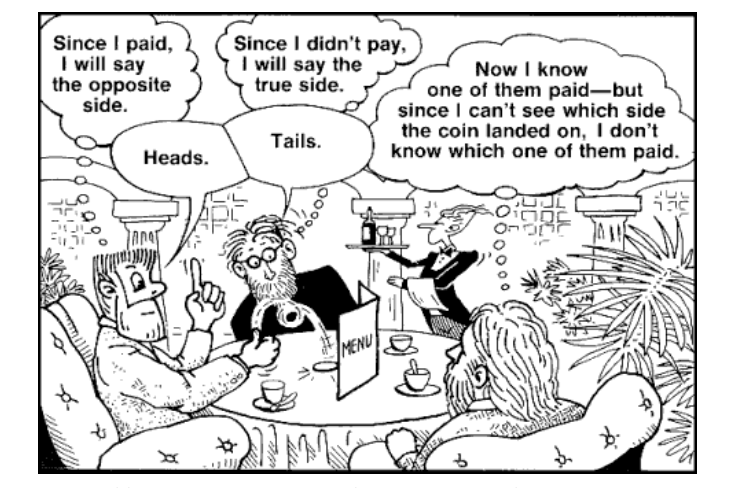
\includegraphics{res/dc.png}
\caption{Dining Cryptographers}\label{fig:dc}
\end{figure}
\textit{DC (Dining Cryptographers) networks allow participants to communicate anonymously by sharing secrets with each other individually.}
\begin{itemize}
  \item \textbf{Use Cases}: Anonymous voting, whistleblowing, and secure communication.
  \item \textbf{Advantages}: Provable anonymity and resistance to traffic analysis.
  \item \textbf{Limitations}: Scalability issues with a large number of participants.
\end{itemize}

\subsection{Blind Messaging Services}
\textit{Replicated databases by different operators are used to enable unobservability of the client request.}
\begin{itemize}
  \item \textbf{Use Cases}: Unobservable database retrieval.
  \item \textbf{Advantages}: Protection from database operators.
  \item \textbf{Limitations}: Requires multiple operators to prevent collusion.
\end{itemize}

\subsection{Mix Networks}
\textit{Mix networks shuffle and encrypt messages at each node to ensure unlinkability between sender and recipient.}
\begin{itemize}
  \item \textbf{Use Cases}: Email anonymization (e.g., Mixminion, Mixmaster), anonymous payments.
  \item \textbf{Advantages}: Strong resistance to traffic analysis, anonymity for sender and recipient.
  \item \textbf{Limitations}: Increased latency, vulnerable to active attacks.
\end{itemize}

\subsection{Integrity Mechanisms}
\begin{itemize}
  \item \textbf{Hash Functions}: Fixed-size digest for verifying data integrity (e.g., SHA-256).
  \item \textbf{Digital Signatures}: Asymmetric encryption for authenticity and non-repudiation.
\end{itemize}

\subsection{Availability Mechanisms}
\begin{itemize}
  \item \textbf{Redundancy}: Use of backup servers and data replication.
  \item \textbf{Load Balancing}:  Distributes network traffic to prevent overload.
  \item \textbf{DDoS Mitigation}:  Techniques like rate limiting and anomaly detection to block malicious traffic.
\end{itemize}



\includepdf[pages={126-161}, nup=4x9]{slides.pdf}
\section{In Practice}

\subsection{IPv6 Traffic Pseudonymization}
\textit{Attacker model is a trusted ISP but untrusted third parties.}
\begin{itemize}
  \item \textbf{Prefix Sharing}: IP addresses are shared between multiple users to create anonymity group. Can lead to collisions, though.
  \item \textbf{Prefix Hopping}: Each customer gets multiple IPs. Trackers cannot link between address changes.
  \item \textbf{Prefix Bouquets}: Each customer uses a different IP for each destination. Trackers cannot link across connections.
\end{itemize}

\subsection{Anonymity Networks in Practice}
\begin{itemize}
  \item \textbf{Tor}: Relays user traffic through multiple nodes to obscure origin and destination. Vulnerable to global adversaries and end-node monitoring.
  \item \textbf{I2P}: Optimized for anonymous communication within the network. Use cases: Peer-to-peer file sharing, messaging, and hosting services.
  \item \textbf{Mix Networks}: Provide stronger anonymity by shuffling and re-encrypting messages at each node. Used in email anonymization and anonymous transactions.
\end{itemize}
\subsection{Other noteworthy topics}
\begin{itemize}
  \item \textbf{Censorship Resistance}: Techniques to bypass network restrictions and surveillance.
  \item \textbf{Misuse of Anonymity}: Use of privacy-enhancing technologies for illicit activities (e.g., illegal marketplaces, malware distribution).
  \item \textbf{Data Retention Policies}: Mandated storage of communication metadata for investigative purposes. Conflict with privacy-focused systems and anonymization techniques.
\end{itemize}



\includepdf[pages={161-216}, nup=4x9]{slides.pdf}
\part{Location Privacy}
\section{Location Privacy \& Mobile Networks}

\subsection{Overview}
\begin{itemize}
  \item \textbf{Objective}: Protect users' location information from being tracked or monitored by adversaries or unauthorized entities.
  \item \textbf{Challenges}: Balancing privacy and utility in location-based services.
\end{itemize}

\subsection{Systematic Protection Methods}
\begin{enumerate}
  \item \textbf{Broadcasting}: Randomized transmission of location data.
  \item \textbf{Group Pseudonyms}: Shared identifiers among a group of users to obscure individual location.
  \item \textbf{Temporal Pseudonyms}: Changing pseudonyms periodically to reduce traceability.
  \item \textbf{Mixing Networks}: Use of cascaded nodes to anonymize the source and destination of location data.
\end{enumerate}

\subsection{Broadcasting Techniques}
\begin{itemize}
  \item \textbf{Implicit Addressing}: Indirectly target devices by broadcasting generalized location updates.
  \item \textbf{Variable Broadcasts}: Adjust broadcast size dynamically to obscure exact location.
\end{itemize}

\subsection{Pseudonyms}
\begin{itemize}
  \item \textbf{Group Pseudonyms}: Shared identifiers among a group of users within region to obscure individual location.
  \item \textbf{Temporal Pseudonyms}: Pseudonyms change over time to prevent long-term tracking.
\end{itemize}

\subsection{Mobile Communication-Mixing}
\begin{itemize}
  \item \textbf{Centralized Approach}: Trusted third party manages pseudonym and location updates. High scalability but susceptible to single points of failure.
  \item \textbf{Decentralized Approach}: Users and mix cascades collaborate to anonymize location updates. Improves privacy but increases coordination complexity.
\end{itemize}

\subsection{Anonymity Techniques in Mobile Networks}
\begin{itemize}
  \item \textbf{Mix Networks}: Shuffle and re-encrypt location data to prevent tracking.
  \item \textbf{Blind Signatures}: Sign messages without revealing the signer's identity.
\end{itemize}

\subsection{Mobile Internet Protocol (IP)}
\begin{itemize}
  \item \textbf{Location Hiding}: Use of proxies or agents to hide the user's exact location.
  \item \textbf{Challenges}: Higher latency due to intermediate nodes. Trade-off between performance and privacy.
\end{itemize}

\subsection{Performance Analysis of Privacy Methods}
\begin{itemize}
  \item \textbf{Trust Levels}: Varying levels of trust required in centralized vs. decentralized systems.
  \item \textbf{Efficiency Loss}: Privacy-preserving methods incur bandwidth and processing overhead (1-10\%).
  \item \textbf{Protection Metrics}: Degree of protection against tracking and profiling varies by method.
\end{itemize}

\end{document}